\documentclass[../main.tex]{subfiles}
\begin{document}
\chapter{Moon Cloud: un framework per il monitoraggio e la security assurance}
\section{Introduzione}
In questo capitolo verrà approfondito Moon Cloud\footnote{MOnitoring and assurance ON Cloud, \textit{https://www.moon-cloud.eu/}}, un framework per il monitoraggio e l'assurance di sistemi tradizionali, cloud e Internet of Things, sviluppato dai ricercatori del laboratorio SESAR Lab\footnote{SEcure Service-oriented Architectures Research Lab - \textit{http://sesar.di.unimi.it}} dell'Università degli Studi di Milano.

L'obiettivo del progetto Moon Cloud è quello di implementare una metodologia automatica per la valutazione della sicurezza, delle performance e di altre proprietà non funzionali, offrendo un processo di assurance basato su attività di auditing e raccolta di evidenze.

Le caratteristiche di Moon Cloud sono le seguenti\cite{MoonCloudWebsite}:
\begin{itemize}
    \item \textbf{Framework automatico e personalizzabile orientato a microservizi} basato su modelli per la raccolta di evidenze
    \item \textbf{Copertura di tutto lo stack cloud}, ai livelli \textit{IaaS}, \textit{PaaS}, \textit{SaaS}
    \item \textbf{Possibilità di integrazione con tecnologie pre-esistenti e di terze parti}
\end{itemize}

L'orchestrazione avviene tramite una  \textit{dashboard} grafica erogata in modalità \textit{Software as-a-Service}, la quale si interfaccia con diversi componenti che ne implementano la logica di funzionamento, l'esecuzione dei test, il collezionamento dei risultati e il reporting dello stato di compliance del sistema analizzato.

L'obiettivo di questo capitolo è quello di dare al lettore il \textit{know-how} necessario a comprendere le motivazioni di alcune decisioni prese nella realizzazione della tesi ed alcune limitazioni del framework Moon Cloud. 
Di seguito sarà proposta una breve panoramica sulla terminologia utilizzata, sulle componenti principali,  e sui principi di funzionamento dei processi di \textit{assessment} e \textit{compliance} all'interno della piattaforma.


\section{Terminologia}
\label{sec:terminology}
\begin{itemize}
    \item \textbf{Metriche}: insieme di proprietà non funzionali di cui si vogliono ottenere \textbf{misurazioni}.
    \item \textbf{Controllo}: rappresenta la modalità di raccolta ed elaborazione delle \textit{misurazioni} di una \textit{metrica}.
        Esso è descritto tramite un documento \textit{JSON}\footnote{JSON, JavaScript Object Notation, \textit{http://www.json.org/}}, i cui attributi sono
        \begin{itemize}
            \item \textbf{name}, nome del controllo
            \item \textbf{description}, descrizione del controllo
            \item \textbf{category}, categoria di appartenenza
            \item \textbf{driver-name}, nome del driver che ne implementa il flusso di esecuzione
            \item \textbf{inputs}, dati ricevuti in input
            \item \textbf{outputs}, dati attesi in output (\textit{misurazioni})
        \end{itemize}
    \item \textbf{Driver}: la porzione di codice che implementa il controllo 
    \item \textbf{Test}: istanza di un controllo, che ne rappresenta l'esecuzione con gli input effettivi 
    \item \textbf{Regola di valutazione astratta}, o \textit{AER (abstract evaluation rule)}, regola logica che implementa un processo di valutazione. È data dall'aggregazione di controlli mediante operatori \textit{booleani}. I suoi termini possono essere \textit{controlli} e altre \textit{AER}.
    \item \textbf{Regola di valutazione concreta}, o \textit{ER (evaluation rule)}: istanza di una \textit{AER}. I suoi termini possono essere \textit{test} (mappati sui rispettivi \textit{controlli} o altre \textit{ER}.
\end{itemize}
\vfill
\newpage

\section{Architettura e componenti}
\begin{figure}[H]
\centering
\makebox[\textwidth]{
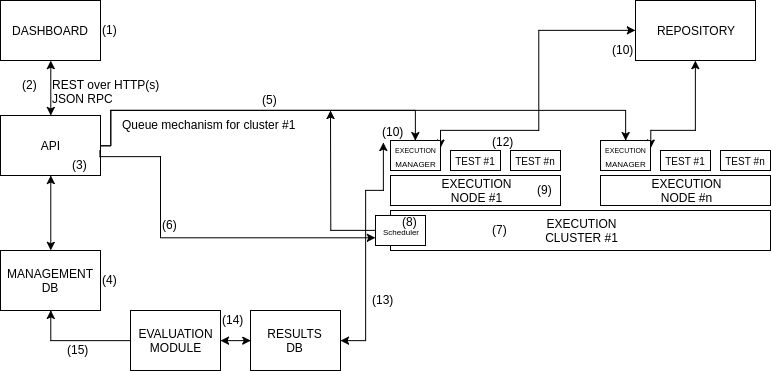
\includegraphics[width=\textwidth]{immagini/MCArchi.png}
}
\caption{Architettura e componenti di Moon Cloud}\label{fig:MCArchi}
\end{figure}
In figura \ref{fig:MCArchi} sono illustrate l'architettura del framework Moon Cloud e l'interazione tra i vari microservizi che lo compongono.
Questa può essere divisa in due aree. La prima, accessibile dagli utenti del sistema fornisce le funzionalità di gestione e comprende:
\begin{itemize}
    \item \textbf{Dashboard} (1), sviluppata in Javascript, HTML5 e CSS mediante il framework Angular.JS. Rappresenta il punto di ingresso per l'utente, e fornisce un'interfaccia grafica per la fruizione delle funzionalità del prodotto. La \textit{Dashboard} è supportata da API HTTP servite in modo sicuro tramite il protocollo TLS (2).
    \item \textbf{API} (3), costituiscono l'intefaccia con le principali funzionalità del sistema. Interagiscono con un database di management (4) seguendo il paradigma RESTful, e orchestrano l'esecuzione dei test.
        Il test può essere lanciato:
        \begin{itemize}
            \item in modalità one-shot, inviando un messaggio agli \textit{execution manager} (9) mediante un meccanismo di comunicazione basato su code(5).
            \item inserendo un \textit{task} periodico(6) nello \textit{scheduler} (7)
        \end{itemize}
        Successivamente alla conclusione del test di sicurezza, \textit{one-shot} o \textit{periodico} che sia, i risultati restituiti saranno disponibili sulla dashboard, con la possibilità di filtrarli e analizzarne le metriche.
\end{itemize}
La seconda invece, rappresenta il vero e proprio backend del framework, gestendo i meccanismi di esecuzione dei test, raccolta dei risultati e valutazione degli stessi.
È composta da:
\begin{itemize}
    \item \textbf{Execution Cluster} (8), ovvero l'insieme dei nodi - \textit{execution node}, (9)  - che eseguono materialmente il test. Gli execution cluster sono equipaggiati da uno \textit{scheduler} (7), che gestisce l'esecuzione temporizzata dei test periodici, per effettuare il monitoraggio in modo continuo, inviando i test in esso memorizzati a cadenze temporali scandite da un pattern \textit{CRON}\footnote{http://man7.org/linux/man-pages/man5/crontab.5.html}.
    \item \textbf{Execution Manager} (10), ovvero il servizio che gestisce il lavoro di ciascun nodo del cluster.        
        Gli \textit{execution manager} di uno stesso cluster sono connessi alla stessa coda: all'arrivo di un messaggio essi effettuano il download il driver relativo al controllo referenziato dal test dal repository (11), eseguono lo stesso con gli input contenuti nel messaggio, e collezionano gli output del test nel \textit{results database}. 
    \item \textbf{Evaluation Module} (13), rimane in ascolto sul database dei risultati (12) in attesa di eventi. Quando lo stato di uno specifico test cambia, avvia la procedura di valutazione di tutte le \textit{ER} che fanno riferimento a tale test, e ne memorizza il risultato nel database di management (4).
    \item \textbf{Repository} (10), contiene i driver per i controlli di sicurezza. È realizzato tramite un ambiente Git\footnote{Git, \textit{https://git-scm.com/}}, di cui condivide le funzionalità, e da un \textit{registry} di \textit{container}, che rappresentano il singolo driver. Il processo di sviluppo di un driver è ultimato da un motore di \textit{continuous integration} che contestualmente al caricamento del codice dello stesso sul \textit{repository} effettua la build del \textit{container} associato e test automatici di validazione e sanitizzazione dello stesso, per poi pubblicare il \textit{container} sul \textit{registry}.
\end{itemize}
\section{Moon Cloud come strumento di verifica delle raccomandazioni}
Mediante i componenti software illustrati nel paragrafo precedente, Moon Cloud è in grado di effettuare un processo di \textit{security assessment} basato sulla verifica di \textit{recommendation}.
Per verifica delle \textit{recommendation} si intende il controllo  della conformità di un sistema target rispetto ad una data raccomandazione.

Si tratta di un processo complesso, che richiede l'aggregazione delle valutazioni di diversi servizi. La tecnica adottata da Moon Cloud consiste nella raccolta di evidenze mediante il testing e il monitoraggio di uno specifico servizio, al fine di verificare se la raccomandazione sia effettivamente rispettata oppure no\cite{MyPaper}.

\begin{definition}[\textbf{Recommendation verification\cite{MyPaper}}]\label{def:prop}
    Sia $\Rec{}$ la \textit{recommendation} da verificare, la \textit{reccomendation verification} è una funzione  $\widehat{\Rec{}}$  definita sulla tupla $\langle$$\EP{}$, $\ER{}$$\rangle$ che restituisce un valore booleano \{true, false\} dove:

\begin{itemize}
    \item $\EP{}$ è l'insieme di \textit{processi di valutazione} \{$\Eval{}$\} da eseguire. L'\textit{output} del processo di valutazione è un valore \textit{booleano} che espreime se la valutazione abbia avuto successo o no, aggregato alle \textit{evidence} collezionate a supporto del risultato.
        \item $\ER{}$ è una \textit{evaluation rule} espressa come formula di logica proposizionale, i cui termini sono i singoli processi di valutazione $\Eval{}$. Essa combina il risultato di vari processi $\Eval{}$$\in$$\EP{}$ e restituisce true se la valutazione ha successo, altrimenti restituisce false.
\end{itemize}
\end{definition}
\begin{definition}[\textbf{Eval\{\}}]\label{def:eval}
    Un processo di valutazione\cite{MyPaper} $Eval\{\}$ è una tupla della forma $\langle$$t$, $C$$\rangle$, dove:
\begin{itemize}
	\item $t$ è il \emph{ToE (Target of Evaluation)}, ovvero i servizi o i meccanismi, che costituiscono il perimetro entro cui la proprietà o la funzionalità di sicurezza deve essere valutata
	\item $C$ è il \emph{Control}, ovvero la funzione di valutazione su $t$ che restituisce il risultato della valutazione insieme a un insieme di evidenze.
\end{itemize}
\end{definition}

Un controllo $C$ specifica i dettagli su come collezionare le evidenze su un target $t$ per valutare la \textit{reccomendation}. È definito nel seguente modo\cite{MyPaper}:


\begin{definition}[\textbf{$C$}]\label{def:control}
    $C$ è definito su una tripla della forma $\langle$$\phi$, $\lambda$, $\pi$$\rangle$, dove:
\begin{itemize}
	\item $\phi$ è il flusso di esecuzione del processo di raccolta  delle evidenze. È composto da una sequenza di operazioni atomiche. 
	\item $\lambda$ è un insieme di \textit{parametri} necessari a collegare il flusso $\phi$ al target $t$ 
	\item $\pi$ è un insieme di \textit{Environmental Settings} che descrivono le caratteristiche dell'ambiente in cui il controllo deve essere eseguito e le possibili dipendenze software dello stesso. 
\end{itemize}
\end{definition}

Moon Cloud è in grado di eseguire molteplici processi di valutazione $ \Eval{} $ in parallelo, ciascuno dei quali si riferisce a un insieme di raccomandazioni $\Rec{}$ che devono essere valutati.
I controlli $C$ sono modellati utilizzando degli schemi, il flusso di esecuzione del codice ($\phi$) è modellato come una catena formata da tutte le operazioni che un controllo necessita di effettuare per raccogliere le evidenze, ed è implementato sotto forma di script Python.
I parametri ($\lambda$) e l'ambiente ($\pi$) sono rappresentati da metadati; ciascuna operazione del flusso $\phi$ è collegata agli specifici parametri necessari per la valutazione, mentre l'ambiente $\pi$ rappresenta l'insieme di prerequisiti e dipendenze che devono persistere per l'esecuzione del controllo\cite{MyPaper}.


\subsection{Regole di valutazione}
Nel contesto implementativo le regole di valutazione sono modellate attraverso le classi \textit{AbstractEvaluationRule} e \textit{EvaluationRule}, rispettivamente per le regole astratte e per le regole concrete.
Di seguito verranno approfondite entrambe le classi.

\subsubsection{Regole di valutazione astratte}
Per la classe \textit{AbstractEvaluationRule} è definita una proprietà \textit{formula} che contiene la formula in logica proposizionale che rappresenta il processo di valutazione.

La formula è espressa in un linguaggio libero dal contesto la cui grammatica è definita tramite la seguente BNF\footnote{BNF, Backus-Naur Form}:
\begin{figure}[H]
\begin{lstlisting}

expressions
    : expr $ 
    ;

expr
    : TOKEN_VAR                       
    | expr TOKEN_AND expr             
    | expr TOKEN_OR expr              
    | expr TOKEN_IMPLIES expr         
    | expr TOKEN_IFF expr             
    | TOKEN_NOT expr 
    | TOKEN_LPAREN expr TOKEN_RPAREN  
    ;


\end{lstlisting}
\end{figure}

I token di questa grammatica sono \textit{variabili} gestite dall'espressione regolare
\begin{itemize}
    \item TOKEN\_VAR $\rightarrow$ \textit{[cf]"\#"\textbackslash d+}
\end{itemize}
e \textit{operatori} (distinguibili in operatori unari e binari a seconda dell'arietà), implementati nel seguente modo: 
\begin{itemize}
    \item TOKEN\_NOT $\rightarrow$ not(expr), operatore unario che effettua la negazione del termine: $return ~ \sim expr$ 
    \item TOKEN\_AND $\rightarrow$ and(expr1, expr2), operatore binario che effettua l'\textit{and} logico dei termini: $return ~ expr1 \wedge expr2$
    \item TOKEN\_OR $\rightarrow$ or(expr1, expr2), operatore binario che effettua l'\textit{or} logico dei termini: $return ~ expr1 \vee expr2$
    \item TOKEN\_IMPLIES $\rightarrow$ implies(term1, term2), operatore binario che implementa l'operatore di implicazione: $return ~ \sim expr1 \vee expr2$
    \item TOKEN\_IFF $\rightarrow$ iff(term1, term2), operatore binario che implementa l'operatore "se e solo se": $return ~ (\sim term1 \vee term2) \wedge (\sim term2 \vee term1)$
\end{itemize}
\textit{TOKEN\_LPAREN} e \textit{TOKEN\_RPAREN} sono rispettivamente la parentesi tonda aperta e chiusa.

Tramite questo linguaggio è possibile generare tutte le formule ben formate della logica proposizionale.

Le variabili possono essere quindi \textit{Controlli} (rappresentati dalla classe \textit{Control}, e indicati nella formula con la sintassi "c\#<id>", dove <id> è l'identificativo del controllo) ed altre \textit{AER} (indicate nella formula, in modo analogo ai controlli, con la sintassi "f\#<id>"). Ciò permette di organizzare le regole di valutazione astratte secondo una gerarchia, concedendo all'utente una maggiore capacità espressiva nel processo di traduzione da politica a regola logica.


\subsubsection{Regole di valutazione concrete}

Le regole di valutazione concrete rappresentano le istanze delle \textit{AER} sopra descritte.
In questo caso la proprietà \textit{formula} è derivata mediante l'applicazione della funzione di mapping $m(\chi)$, \eqref{function:mapping} dove $\chi$ è la regola di valutazione astratta di partenza, $c_i$ è un controllo, $t_i$ è un test ed $e$ è una regola di valutazione concreta.
\begin{equation}
\begin{gathered}
m(\chi):
c \rightarrow t ~ \forall c_i \in \chi ~ | ~ t ~ \text{refers} ~ c ~ \text{\textbf{,}} ~
        f \rightarrow e ~ \forall \chi_i \in \chi ~ | ~ e ~ \text{refers} ~ \chi_i
\end{gathered}
\label{function:mapping}
\end{equation}
Tutte le regole di valutazione astratte incluse nella regola di partenza sono quindi sostituite da una o più regole di valutazione concrete che le referenziano, analogamente tutti i controlli inclusi nella regola di partenza sono sostituiti da uno o più test.
Il mapping avviene sulla base di un oggetto JSON \textit{chiave-valore}, in cui la chiave rappresenta l'identificativo dell'elemento di partenza e il valore rappresenta l'identificativo dell'elemento di arrivo.

La grammatica utilizzata per la validazione della formula così derivata, è ovviamente analoga alla precedente, ad eccezione del token \textit{TOKEN\_VAR} che assume valori rappresentabili dalla seguente espressione regolare:
\begin{center}
    TOKEN\_VAR $\rightarrow$ \textit{[et]"\#"\textbackslash d+}
\end{center}
supportando il carattere '\textit{e}' per indicare le Evaluation Rule, e il carattere '\textit{t}' per indicare i test.
In fase di esecuzione del processo di valutazione sarà questa la formula effettivamente utilizzata, sostituendo a ciascun termine il valore booleano del test o dell'evaluation rule referenziata.
\vfill
\newpage
\subsection{Driver per i controlli di sicurezza}
Di seguito verrà illustrata la struttura di un driver Moon Cloud, utilizzato per l'implementazione effettiva dei controlli di sicurezza e per l'esecuzione dei test.

I driver sono costituiti da container \textit{Docker} basati sull'immagine \textit{python:2-onbuild}\footnote{https://hub.docker.com/\_/python/} e possono essere eseguiti sia all'interno del framework Moon Cloud che in modalità completamente standalone.
Il container è gestito da un \textit{entrypoint} che riceve gli input per l'esecuzione del test, colleziona eventuali log di diagnostica e restituisce gli output all'\textit{Execution Manager}.
Sia l'input che l'output di un driver sono costituiti da documenti JSON le cui chiavi devono corrispondere a quelle dichiarate negli attributi \textit{inputs} e \textit{outputs}, del \textit{Controllo} corrispondente, precedentemente trattati nella sezione \ref{sec:terminology}
\subsubsection{Struttura di un driver}
\label{subsec:strutturadriver}
All'interno del container sono presenti due componenti:
\begin{itemize}
    \item{\textit{entrypoint.py}}, il cui ruolo è quello di leggere ed effettuare la deserializzazione degli \textit{input}, leggere i metadati del driver, e precaricare la classe del driver.
        Il discovery della classe viene fatto in modo automatico da una directory chiamata \textit{test/} che andremo a dettagliare tra poco.
    \item{\textit{driver.py}}, che fornisce un'\textit{interfaccia} mediante la classe \textit{Driver} che ciascun payload dovrà implementare.
        Una peculiarità della classe \textit{Driver} è la presenza della sottoclasse \textit{\_\_metaclass\_\_} che fornisce un meccanismo di \textit{subscription} per tutte le classi che ereditano da Driver. Questo permette di far funzionare il meccanismo di \textit{autodiscovery}, permettendo a chi scrive il payload di lavorare in modo agnostico rispetto alle funzionalità del framework.
        L'esecuzione effettiva del codice avviene per mezzo del metodo \textit{run} e un meccanismo di gestione delle operazioni atomiche in due flussi (forward e rollback) dettagliatamente illustrati nella sezione successiva.
        Un'altra classe molto importante è la classe \textit{DriverResult} che fornisce la possibilità di restituire le misurazioni effettuate dal controllo in forma \textit{chiave-valore}.
\end{itemize}

Altri due file molto importanti sono:
\begin{itemize}
    \item \textit{Dockerfile}, che costituisce la definizione di ogni container Docker. Questo permette di installare o compilare eventuali dipendenze software utili all'esecuzione del driver 
    \item \textit{requirements.txt}, che, in Python, contiene tutte le librerie del database PyPI\footnote{https://pypi.python.org/} da cui il codice del driver dipende.
\end{itemize}


\subsubsection{Payload del driver}

\label{subsec:payload}
Il payload del driver è contenuto nella directory \textit{test}, ed è costituito da una classe che eredita la classe \textit{Driver} illustrata in \ref{subsec:strutturadriver} e ne implementa il metodo di interfaccia \textit{appendAtomics}.

Esso è definito da:
\begin{itemize}
\item una sequenza $A$ di $n$ operazioni atomiche $o_n$, con corrispondenza biunivoca con le chiavi specificate nel documento JSON di input
\begin{align*}
A = \{ o_0, o_1, o_2, ... , o_n \}
\end{align*}
\item una sequenza di $n$ operazioni di rollback - una per ogni operazione atomica - che svolgono azioni di \textit{undo}
\begin{align*}
R = \lnot A = \{ r_0, r_1, r_2, ... , r_n \}
\end{align*}
\end{itemize}
aggregati in coppie ordinate.
\begin{align*}
P = \{ (o_0, r_0), (o_1, r_1) , (o_2, r_2) , ... , (o_n, r_n)\}
\end{align*}
Ogni operazione atomica $o_x \in A$ riceve in input gli output dell'operazione $o_{x-1}$; analogamente ogni operazione $r_x$ di rollback $r \in R$ riceve in input gli output di $r_{x+1}$.

\begin{align*}
R_1 \subseteq R =\{ r_{x-1}, r_(x-2), ... , r_{x-n}\}
\end{align*}
\begin{figure}[H]
 \begin{minipage}[b]{6cm}
   \centering
   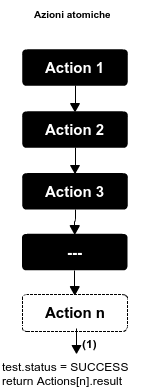
\includegraphics[width=4cm]{immagini/FlowchartProbeOk.png}
   \caption{Esecuzione corretta di un test}\label{fig:probeOk}
 \end{minipage}
 \ \hspace{2mm} \hspace{3mm} \
 \begin{minipage}[b]{9cm}
  \centering
   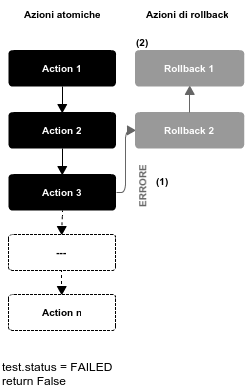
\includegraphics[width=6.6cm]{immagini/FlowchartProbeRollback.png}
   \caption{Esecuzione di un test con operazioni di rollback}\label{fig:probeRb}
 \end{minipage}
\end{figure}
Nella figura \ref{fig:probeOk} è mostrata l'esecuzione di un driver di sonda il cui test viene eseguito correttamente.
Il risultato dell'ultima operazione atomica deve essere un valore \textit{boolean} e viene utilizzato come risultato finale (1).

In caso di fallimento di un'operazione $o_x \in P$ , $x \leq n$ (figura \ref{fig:probeRb}) (1) l'interfaccia della classe \textit{Driver} si occupa di lasciare il sistema target in uno stato sicuro provvedendo ad eseguire in sequenza le operazioni di rollback e restituendo come risultato \textit{False}.

Gli  input globali del test sono  disponibili interrogando la proprietà "\textit{testinstances}", un dizionario a due livelli che contiene nella chiave di primo livello il nome della fase a cui l'input è riferito, nella chiave di secondo livello il nome della chiave del valore di input.

\begin{python}

from driver import Driver
from time import sleep

class MyDriver(Driver):
    def step1(self, inputs):
        self.logger.info("Sto eseguendo lo step 1")
        sleep(10)
        self.logger.info("Ho eseguito lo step 1")
        return True

    def rollback1(self, inputs):
        self.logger.info("Sto eseguendo il rollback dello step 1")
        sleep(10)
        self.logger.info("Ho eseguito il rollback per lo step 1")

    def step2(self, inputs):
        self.logger.info("Sto eseguendo lo step 2")
        self.logger.info("Stampo gli input del test")
        self.logger.info(json.dumps(self.testinstances))
        sleep(10)
        self.logger.info("Ho eseguito lo step 2")
        
    def rollback2(self, inputs):
        self.logger.info("Sto eseguendo il rollback per lo step 2")
        sleep(10)        
        self.logger.info("Ho eseguito il rollback per lo step 2")

    def appendAtomics(self):
        self.appendAtomic(self.step1, self.rollback1)
        self.appendAtomic(self.step2, self.rollback2)
        
\end{python}

Nella directory "test", oltre al payload del driver, è contenuto un file \textit{metadata.json} 
con le seguenti chiavi:
\begin{itemize}
    \item driver-name, nome del driver
    \item inputs, oggetto di cui le chiavi costituiscono il nome simbolico da associare all'input e i valori costituiscono il tipo di dato atteso (stringa, intero ed eventuali tipi di dato personalizzati, anche complessi, come indirizzo ip, account Amazon, account OpenStack)
    \item outputs, oggetto analogo ad inputs, ma per la gestione degli output 
    \item schema, oggetto contenente lo JSON schema utilizzato per effettuare il rendering del form di input nella dashboard
\end{itemize}

\section{Esempio}

Verrà di seguito proposto un esempio per illustrare la definizione completa di un processo di valutazione all'interno della piattaforma Moon Cloud.
La proprietà analizzata da questo esempio è la \textit{confidenzialità del dato} ottenuta dall'aggregazione in \textit{and} logico di due diversi controlli:
\begin{enumerate}
    \item{Confidenzialità dello storage (\textit{c\#1})}
    \item{Confidenzialità del canale di comunicazione (\textit{c\#2})}
\end{enumerate}

\subsection{Abstract Evaluation Rule}
\framebox[\textwidth][l]{\texttt{c\#1 and c\#2}}

\begin{js}
{
    "id":1,
    "name":"Data Confidentiality",
    "description":"It allows to execute a set of tests against a given service to ensure that information are provided over a secure channel and stored over a secure storage.",
    "category":[],
    "formula":"c#1 and c#2",
    "enforced_control":null,
    "enforced_operator":null,
    "cardinality":null,
    "related_controls":[1, 2],
    "related_aers":[],
    "metadata":null
}
\end{js}


\subsection{Controllo}

\subsubsection{Confidenzialità dello storage}

\begin{js}
{
  "category" : [  ],
  "driver" : "storage-confidentiality",
  "id" : 1,
  "metadata" : {
      "description" : "Evaluates storage confidentiality for a given target",
      "schema" : {
          "config" : {
              "properties" : {
                  "ssh_string" : {
                      "title" : "SSH Connection String",
                      "type" : "string"
                    },
                  "ssh_key" : {
                      "title" : "SSH Key",
                      "type" : "string"
                    },
                    "device_to_check": {
                        "title": "Device to check",
                        "type":"string",
                        "default": "/dev/sda"
                    }
                },
              "title" : "Target",
              "type" : "object"
            }
        },
        "inputs": {
            "config": {
                "ssh_string": "string",
                "ssh_key": "string",
                "device_to_check": "string",
            }
        },
        "outputs": {
            "result": "boolean"
        }
    },
  "name" : "Checks luks is enabled on target"
}
\end{js}

\subsubsection{Confidenzialità del canale}

\begin{js}
{
  "category" : [  ],
  "driver" : "channel-confidentiality",
  "id" : 1,
  "metadata" : {
      "description" : "Evaluates SSL configuration for a given target",
      "schema" : {
          "config" : {
              "properties" : {
                  "host" : {
                      "title" : "Host",
                      "type" : "string"
                    },
                  "port" : {
                      "default" : 80,
                      "title" : "port",
                      "type" : "number"
                    }
                },
              "title" : "Target",
              "type" : "object"
            }
        },
        "inputs": {
            "config": {
                "host": "hostname",
                "port": "integer"
            }
        },
        "outputs": {
            "result": "boolean",
            "strength": "string"
        }
    },
  "name" : "Check channel confidentiality"
}
\end{js}






\subsection{Evaluation Rule}
\framebox[\textwidth][l]{\texttt{t\#1 and t\#2}}

\begin{js}
  {
    "aer" : 1,
    "description" : "Checks storage confidentiality and network confidentiality on the target tufarolo.eu",
    "id" : 1,
    "mapping" : {
        "c#1":"t#1",
        "c#2":"t#2"
    },
    "name" : "Confidentiality tufarolo.eu",
    "related_ers" : [  ],
    "related_tests" : [ 1, 2 ],
    "status" : 0,
  }
\end{js}




\subsection{Test}
\subsubsection{Confidenzialità dello storage}
\begin{js}
 {
    "control" : 1,
    "description" : "",
    "execution_cluster" : 1,
    "id" : 11,
    "name" : "",
    "testcase" : {
            "config" : {
                "ssh_string" : "user@tufarolo.eu:22",
                "ssh_key" : ".....",
                "device_to_check": "/dev/sda1"
            }
      },
    "__unicode__" : "t#1"
  }
  \end{js}

\subsubsection{Confidenzialità del canale}
\begin{js}
 {
    "control" : 2,
    "description" : "",
    "execution_cluster" : 1,
    "id" : 11,
    "name" : "",
    "testcase" : {
        "config" : {
            "host" : "tufarolo.eu",
            "port" : 80
          } },
    "__unicode__" : "t#2"
  }


\end{js}

\subsection{Driver}

\subsubsection{Confidenzialità dello storage}
\begin{python}
from driver import Driver
from libraries import ssh
class StorageConfidentiality(Driver):
    def connect_to_ssh(self, inputs):
    ssh.connect(self.testinstances.get("ssh").get("ssh_string"), self.testinstances..get("ssh").get("ssh_key")))
    
    def check_is_luks(self, inputs):
        return ssh.run("/bin/cryptsetup isLuks \%s" \% self.testinstances.get())

    def appendAtomics(self):
        self.appendAtomic(self.connect_to_ssh, lambda(x): None)
        self.appendAtomic(self.check_is_luks, lambda(x): None)

\end{python}

\subsubsection{Confidenzialità del canale}

\begin{python}
from driver import Driver
from libraries import ssl
class ChannelConfidentiality(Driver):
    def check_ssl(self, inputs):
        target = self.testinstances.get("config").get("target")
        port = self.testinstances.get("port").get("port")
        status, strength =  ssl.check(target, port)
        self.result.data["strength"] = strength
        return status
    def appendAtomics(self):
        self.appendAtomic(self.check_ssl, lambda(x): None)

\end{python}



\end{document}
